\section{Implementierung}

In diesem Kapitel wird die Implementierung des Projektes mit Fokussierung auf die einzelnen Komponenten beschrieben.

\subsection{Kommunikation}

Die Kommunikation der einzelnen Komponenten des Schwarmverhaltens baut auf einer klar definierten Struktur, um ein verteiltes System zu ermöglichen, siehe \ref{fig:full_classdiagram}. Die Daten werden dabei als \gls{json} Objekte zur optimalen plattformübergreifenden Interpretation versendet, wobei jeweils die entsprechende Bibliothek zur Serialisierung verwendet wird.
\begin{verbatim}
\end{verbatim}
\begin{figure}[h]
	\begin{center}
		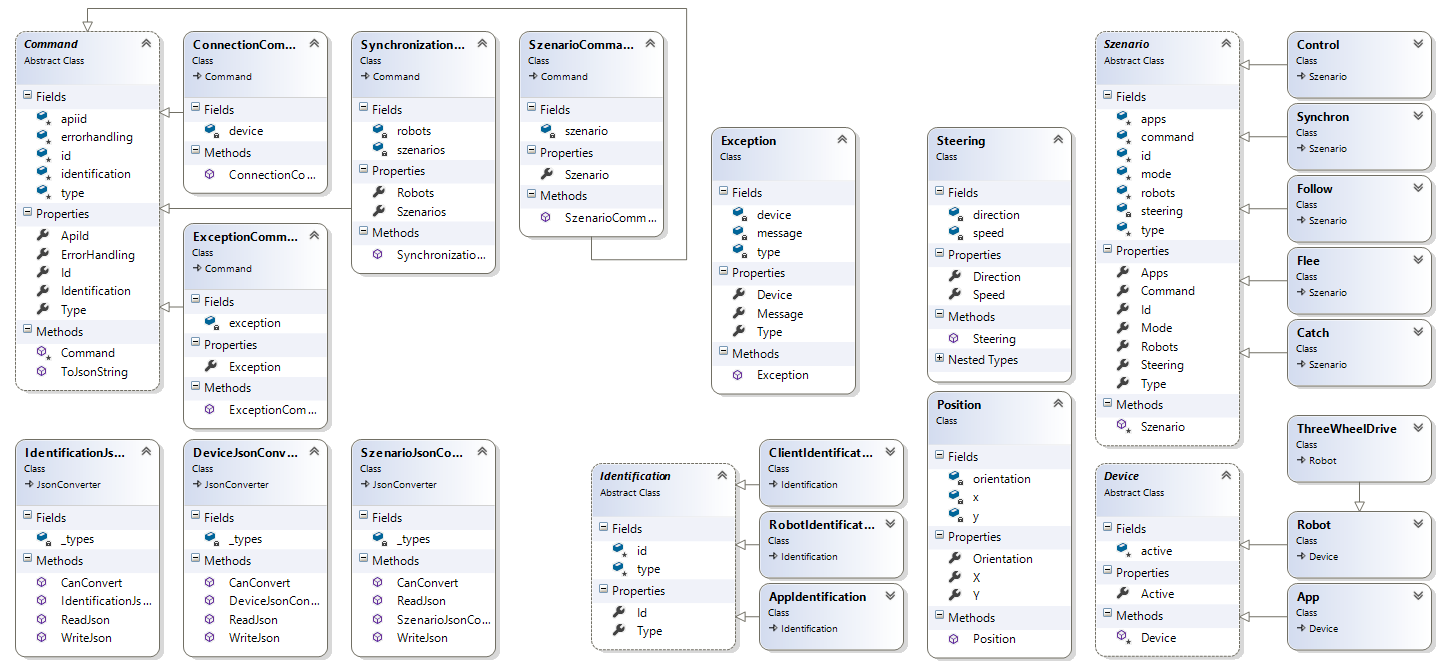
\includegraphics[width=0.95\textwidth]{images/uml/full_class_diagram.png}
	\end{center}
	\caption{Aufbau Commands}
	\label{fig:full_classdiagram}
\end{figure}

\newpage
\noindent
Der Kern zur Implementierung der Kommunikation erfolgt in zwei Methoden, die auf jeder Komponente zur Verfügung stehen. Diese dienen zum Versenden, sowie Empfangen von Daten, wobei diese als Zeichenkette serialisiert und in Bytes aufgeteilt werden, siehe Abbildung \ref{fig:SendCommand}. Um den vollständigen Umfang der Daten zu erfassen, wird die Größe ermittelt und standardmäßig mittels vier Bytes übertragen. Dadurch ist eine maximale Paketgröße von 32 Byte möglich, was einer Länge von etwa 4 Milliarden Zeichen entspricht. Die Interpretation zum Empfangen erfolgt mit ähnlichem Muster, indem zunächst die Größe der Daten festgestellt wird und die Daten deserialiert werden, siehe Abbildung \ref{fig:ReceiveCommand}.

\begin{figure}[h]
	\centering
	\subfloat[Versende Kommando]{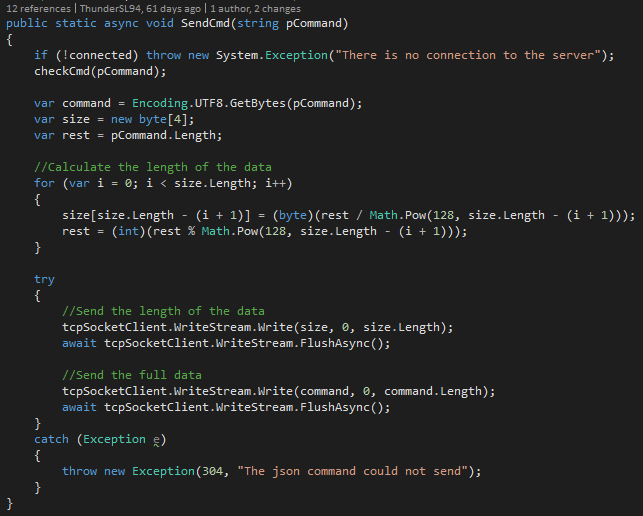
\includegraphics[width=0.6\textwidth]{images/code/SendCommand.png}\label{fig:SendCommand}}
	\qquad
	\subfloat[Empfange Kommando]{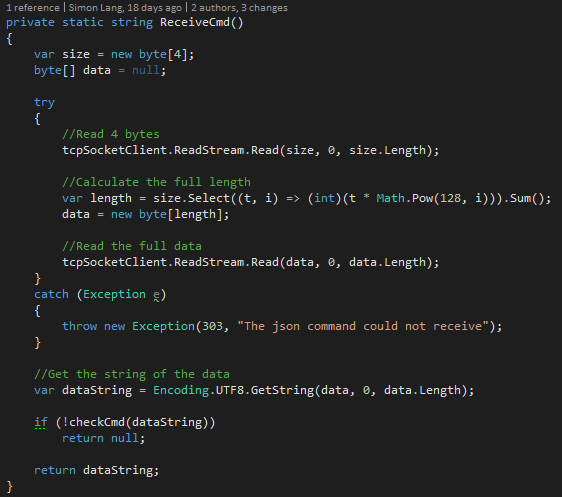
\includegraphics[width=0.6\textwidth]{images/code/ReceiveCommand.png}\label{fig:ReceiveCommand}}
	\caption{Kommunikation}
\end{figure}

\newpage
\paragraph{Kommandos}

\begin{wrapfigure}{r}{0.55\textwidth}
	\begin{center}
		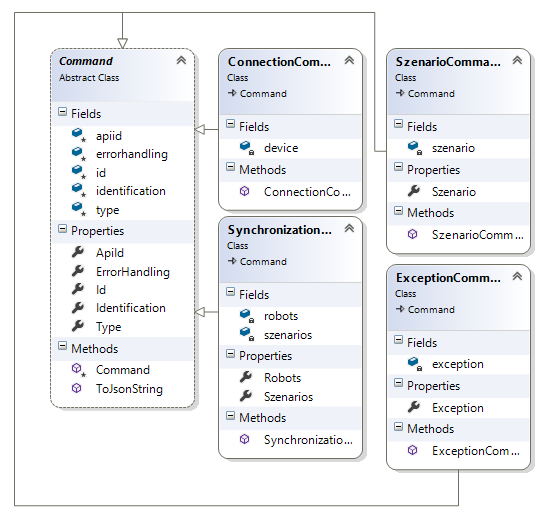
\includegraphics[width=0.5\textwidth]{images/uml/commands.png}
	\end{center}
	\caption{Kommandos}
	\label{fig:commands_classdiagram}
	\begin{center}
		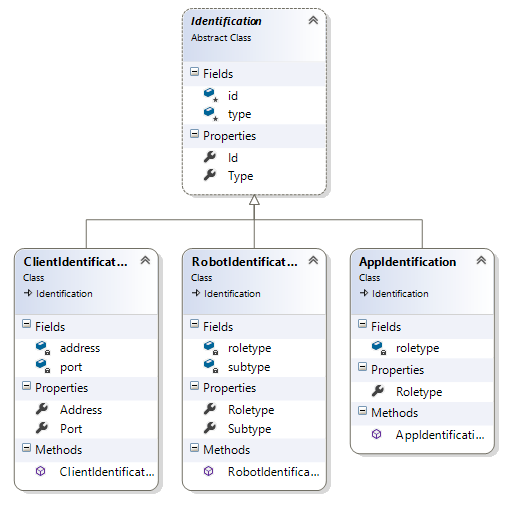
\includegraphics[width=0.5\textwidth]{images/uml/identification.png}
	\end{center}
	\caption{Identifikation}
	\label{fig:identification_classdiagram}
\end{wrapfigure}

stellen die Basis der Kommunikationsstruktur sowie den aktuellen Kontext dar, indem sich die Software befindet, siehe \ref{fig:commands_classdiagram}. Sie enthalten grundlegende Attribute zur allgemeinen Identifikation des Kommandos, die zur Interpretation verwendet, welche über definierte Enums ausgewählt werden. Je nach Kommando sind zusätzliche Objekte enthalten, die durch die jeweilige Id vordefiniert sind.\\

\paragraph{Identifikationen}

stellt die individuelle Identität der einzelnen Komponente dar, siehe \ref{fig:identification_classdiagram}. Diese wird durch eine fortlaufende Identifikationsnummer, Typen und je nach Ableitung weiteren Attributen erreicht. Um die jeweiligen Kommandos entsprechend zuzuordnen, sind diese in jedem Kommando vorhanden und bilden die Basisobjekte. Die unterschiedlichen Typen sind dabei für verschiedene Kontexte der Software zuständig. Die ClientIdentification stellt einerseits die Verbindung einer allgemeinen Komponente zur Desktopanwendung dar, wogegen die Robot- bzw. AppIdentification die spezifische Identifikation der Komponente darstellt. Die Erstellung der Identifikation erfolgt wiederholt zur Anmeldung der Komponente am System. Zunächst wird ein leeres Objekt erzeugt, dass anschließend durch abfragende Kommandos an die entsprechende Komponente befüllt wird, welche hinterher eine berechnete Identifikationsnummer erhält.

\newpage
\paragraph{Geräte}

\begin{wrapfigure}{r}{0.55\textwidth}
	\begin{center}
		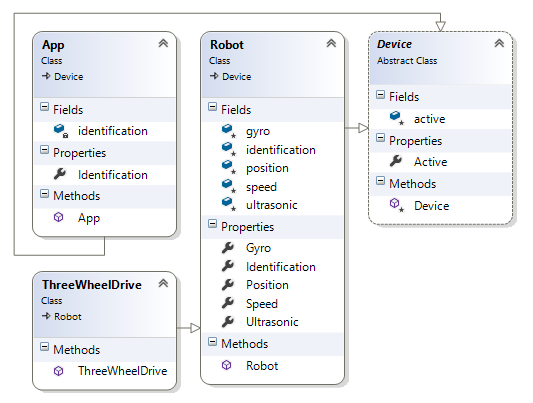
\includegraphics[width=0.5\textwidth]{images/uml/devices.png}
	\end{center}
	\caption{Devices}
	\label{fig:devices_classdiagram}
	\begin{center}
		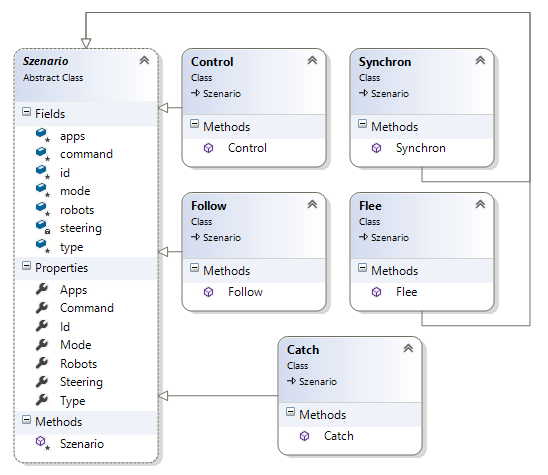
\includegraphics[width=0.5\textwidth]{images/uml/szenarios.png}
	\end{center}
	\caption{Scenarios}
	\label{fig:szenarios_classdiagram}
\end{wrapfigure}

stellen die Komponenten dar, die an einem Szenario eines Schwarmverhaltens teilnehmen, siehe \ref{fig:devices_classdiagram}. Sie enthalten jeweils spezifische Identifikations Objekte, zur gegenseitigen Zuordnung, sowie die erfassten Daten der entsprechenden Systeme. Die Unterscheidung erfolgt in zwei Komponenten, dem Robot und der App, wobei der Roboter in die jeweiligen Untertypen gegliedert werden kann. 

\paragraph{Szenarios}

stellen den aktuellen Kontext des Schwarmverhaltens dar, in dem sich der Nutzer befindet, siehe \ref{fig:szenarios_classdiagram}. Sie enthalten die jeweiligen Teilnehmer des Szenarios, sowie die Steuerungsinformationen und damit die gesamten Daten des aktuellen Kontextes. Diese Objekte werden laufend aktualisiert und besitzen lediglich zur Laufzeit des Szenarios ihre Gültigkeit, wobei diese anschließend gelöscht werden.


%Die Szenarios stellen den aktuellen Kontext des Schwarmverhaltens dar und enthalten zu Identifikations Attributen zusätzliche %die teilnehmenden Devices um diese zuordnen zu könnn. Diese Objekte werden laufend aktualisiert und haben nur zur Laufzeit des %entsprechenden Szenarios ihre Gültigkeit, wobei sie bei Beendigung gelöscht werden.

\newpage
\paragraph{Konverter}
\begin{wrapfigure}{r}{0.55\textwidth}
	\begin{center}
		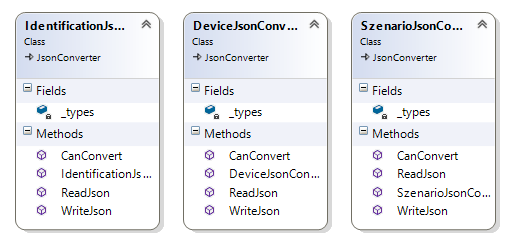
\includegraphics[width=0.5\textwidth]{images/uml/json_converter.png}
	\end{center}
	\caption{JSON Converter}
	\label{fig:converter_classdiagram}
\end{wrapfigure}

Um Objekte spezifisch zu abstrahieren, werden sogenannte Converter verwendet, um abstrahierte Objekte direkt abgeleiteten Klassen zuzuordenn und entsprechende Programmlogik auszuführen. Dabei wird auf die entsprechende Bibliothek mit Grundlogik zurückgegriffen und entsprechende Bedingungen hinzugefügt. siehe \ref{fig:converter_classdiagram}



\newpage
\subsection{App}

\subsubsection{Workflow} %Struktur

\paragraph{Design Pattern}
\paragraph{\acrfull{mvvm}}
\paragraph{Bindings}

\subsubsection{\acrfull{gui}} %Oberfläche

\subsubsection{Buisnesslogic} %Logik

\subsection{Backend}

\begin{comment}
Aufbau
Interpreter
Mechanismen
GUI
\end{comment}

\subsection{Robot}

\begin{comment}
Aufbau
Robot
RobotController
EV3 Library
GUI
\end{comment}